\section{局所探索アルゴリズムの実装}

\begin{frame}{施設配置問題に対する改良された局所探索アルゴリズム}
  \begin{theorem}[\cite{charikar2005improved}]
    施設配置問題に対して，任意の定数 \(\varepsilon > 0\) に対し，
    % \alert{\(\tilde{\mathcal{O}}(n^2/\varepsilon)\)}
    入力と \(1/\varepsilon\) の多項式時間で \alert{\(1 + \sqrt{2} + \varepsilon\)} 倍の近似解を求めるスキームが存在する．
  \end{theorem}

  \textbf{Key Ideas. }
  \begin{columns}
    \begin{column}{0.45\textwidth}
      \begin{itemize}
        \item 開設コストを適切にスケール
      \end{itemize}
      \begin{figure}
        \centering
        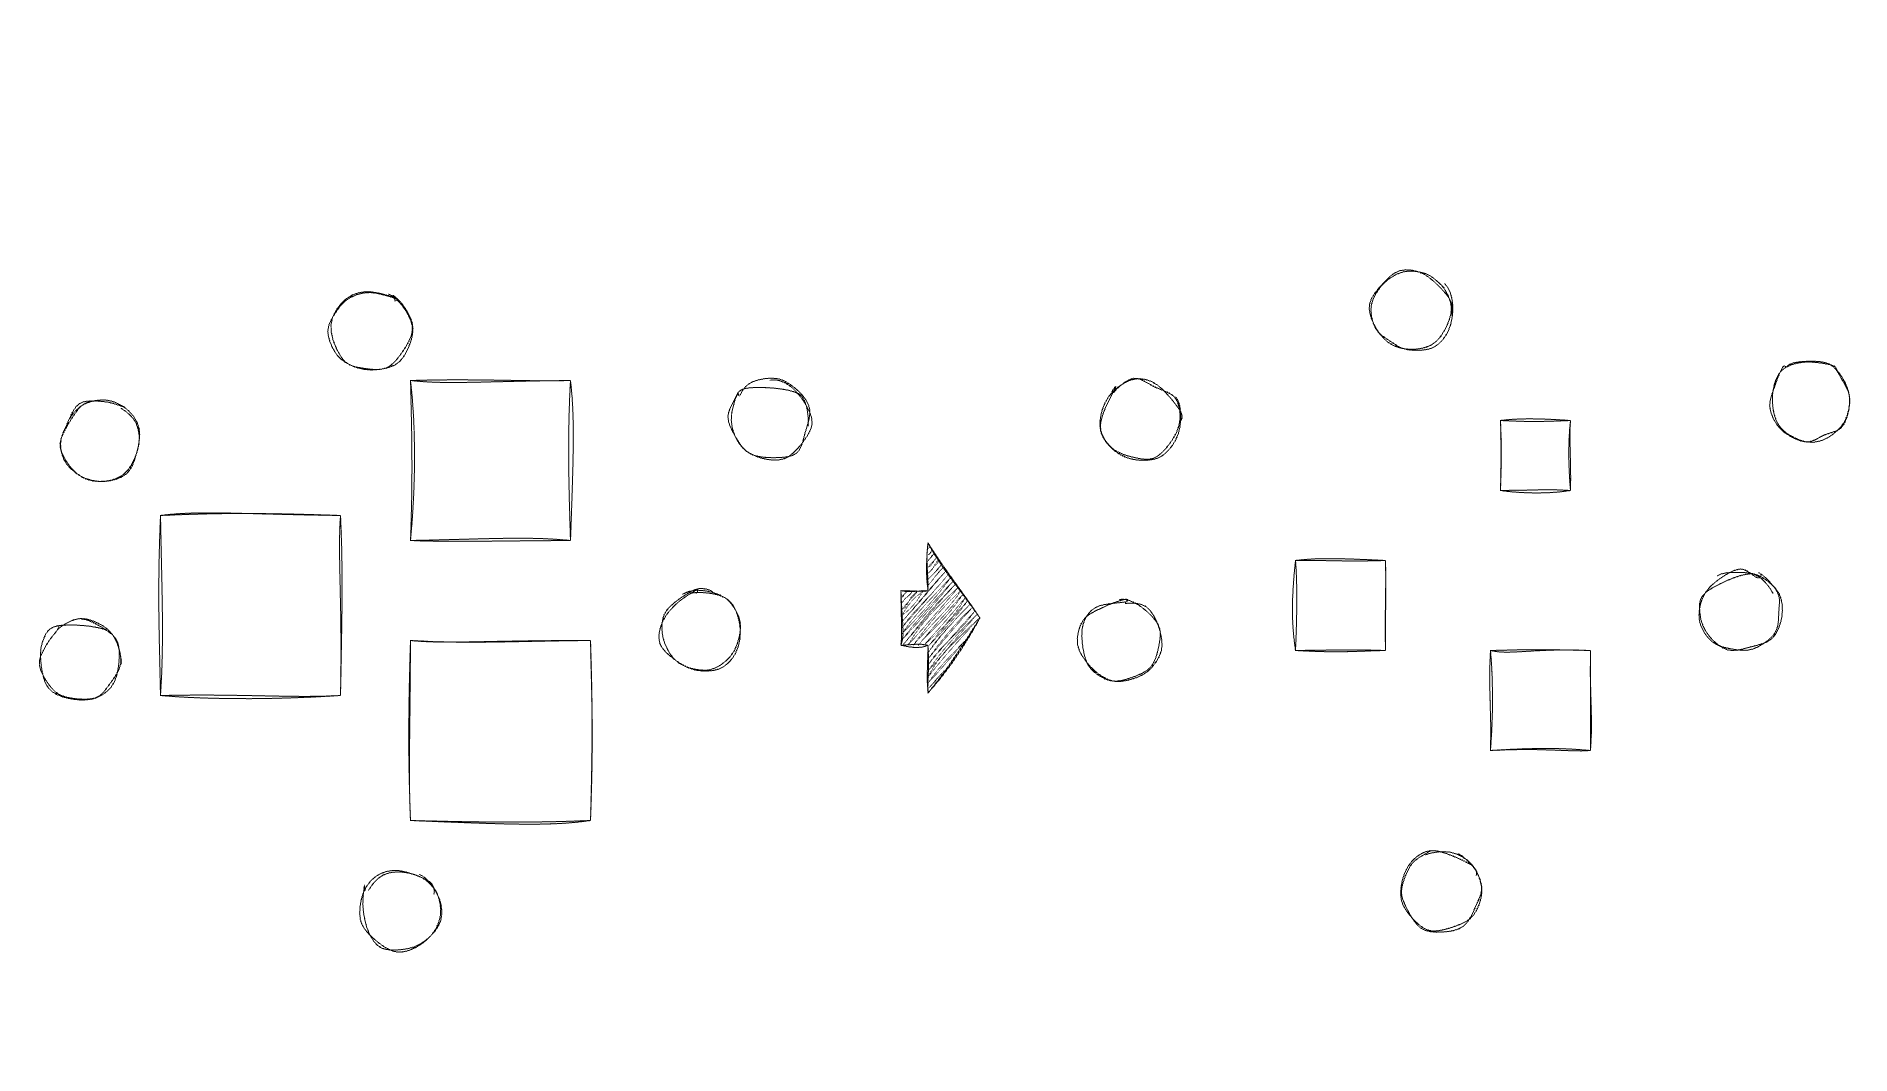
\includegraphics[width=\textwidth]{figures/scheme/scaling.drawio.png}
      \end{figure}
    \end{column}
    \begin{column}{0.45\textwidth}
      \begin{itemize}
        \item 近傍への移動に閾値を設定する
      \end{itemize}
      \begin{figure}
        \centering
        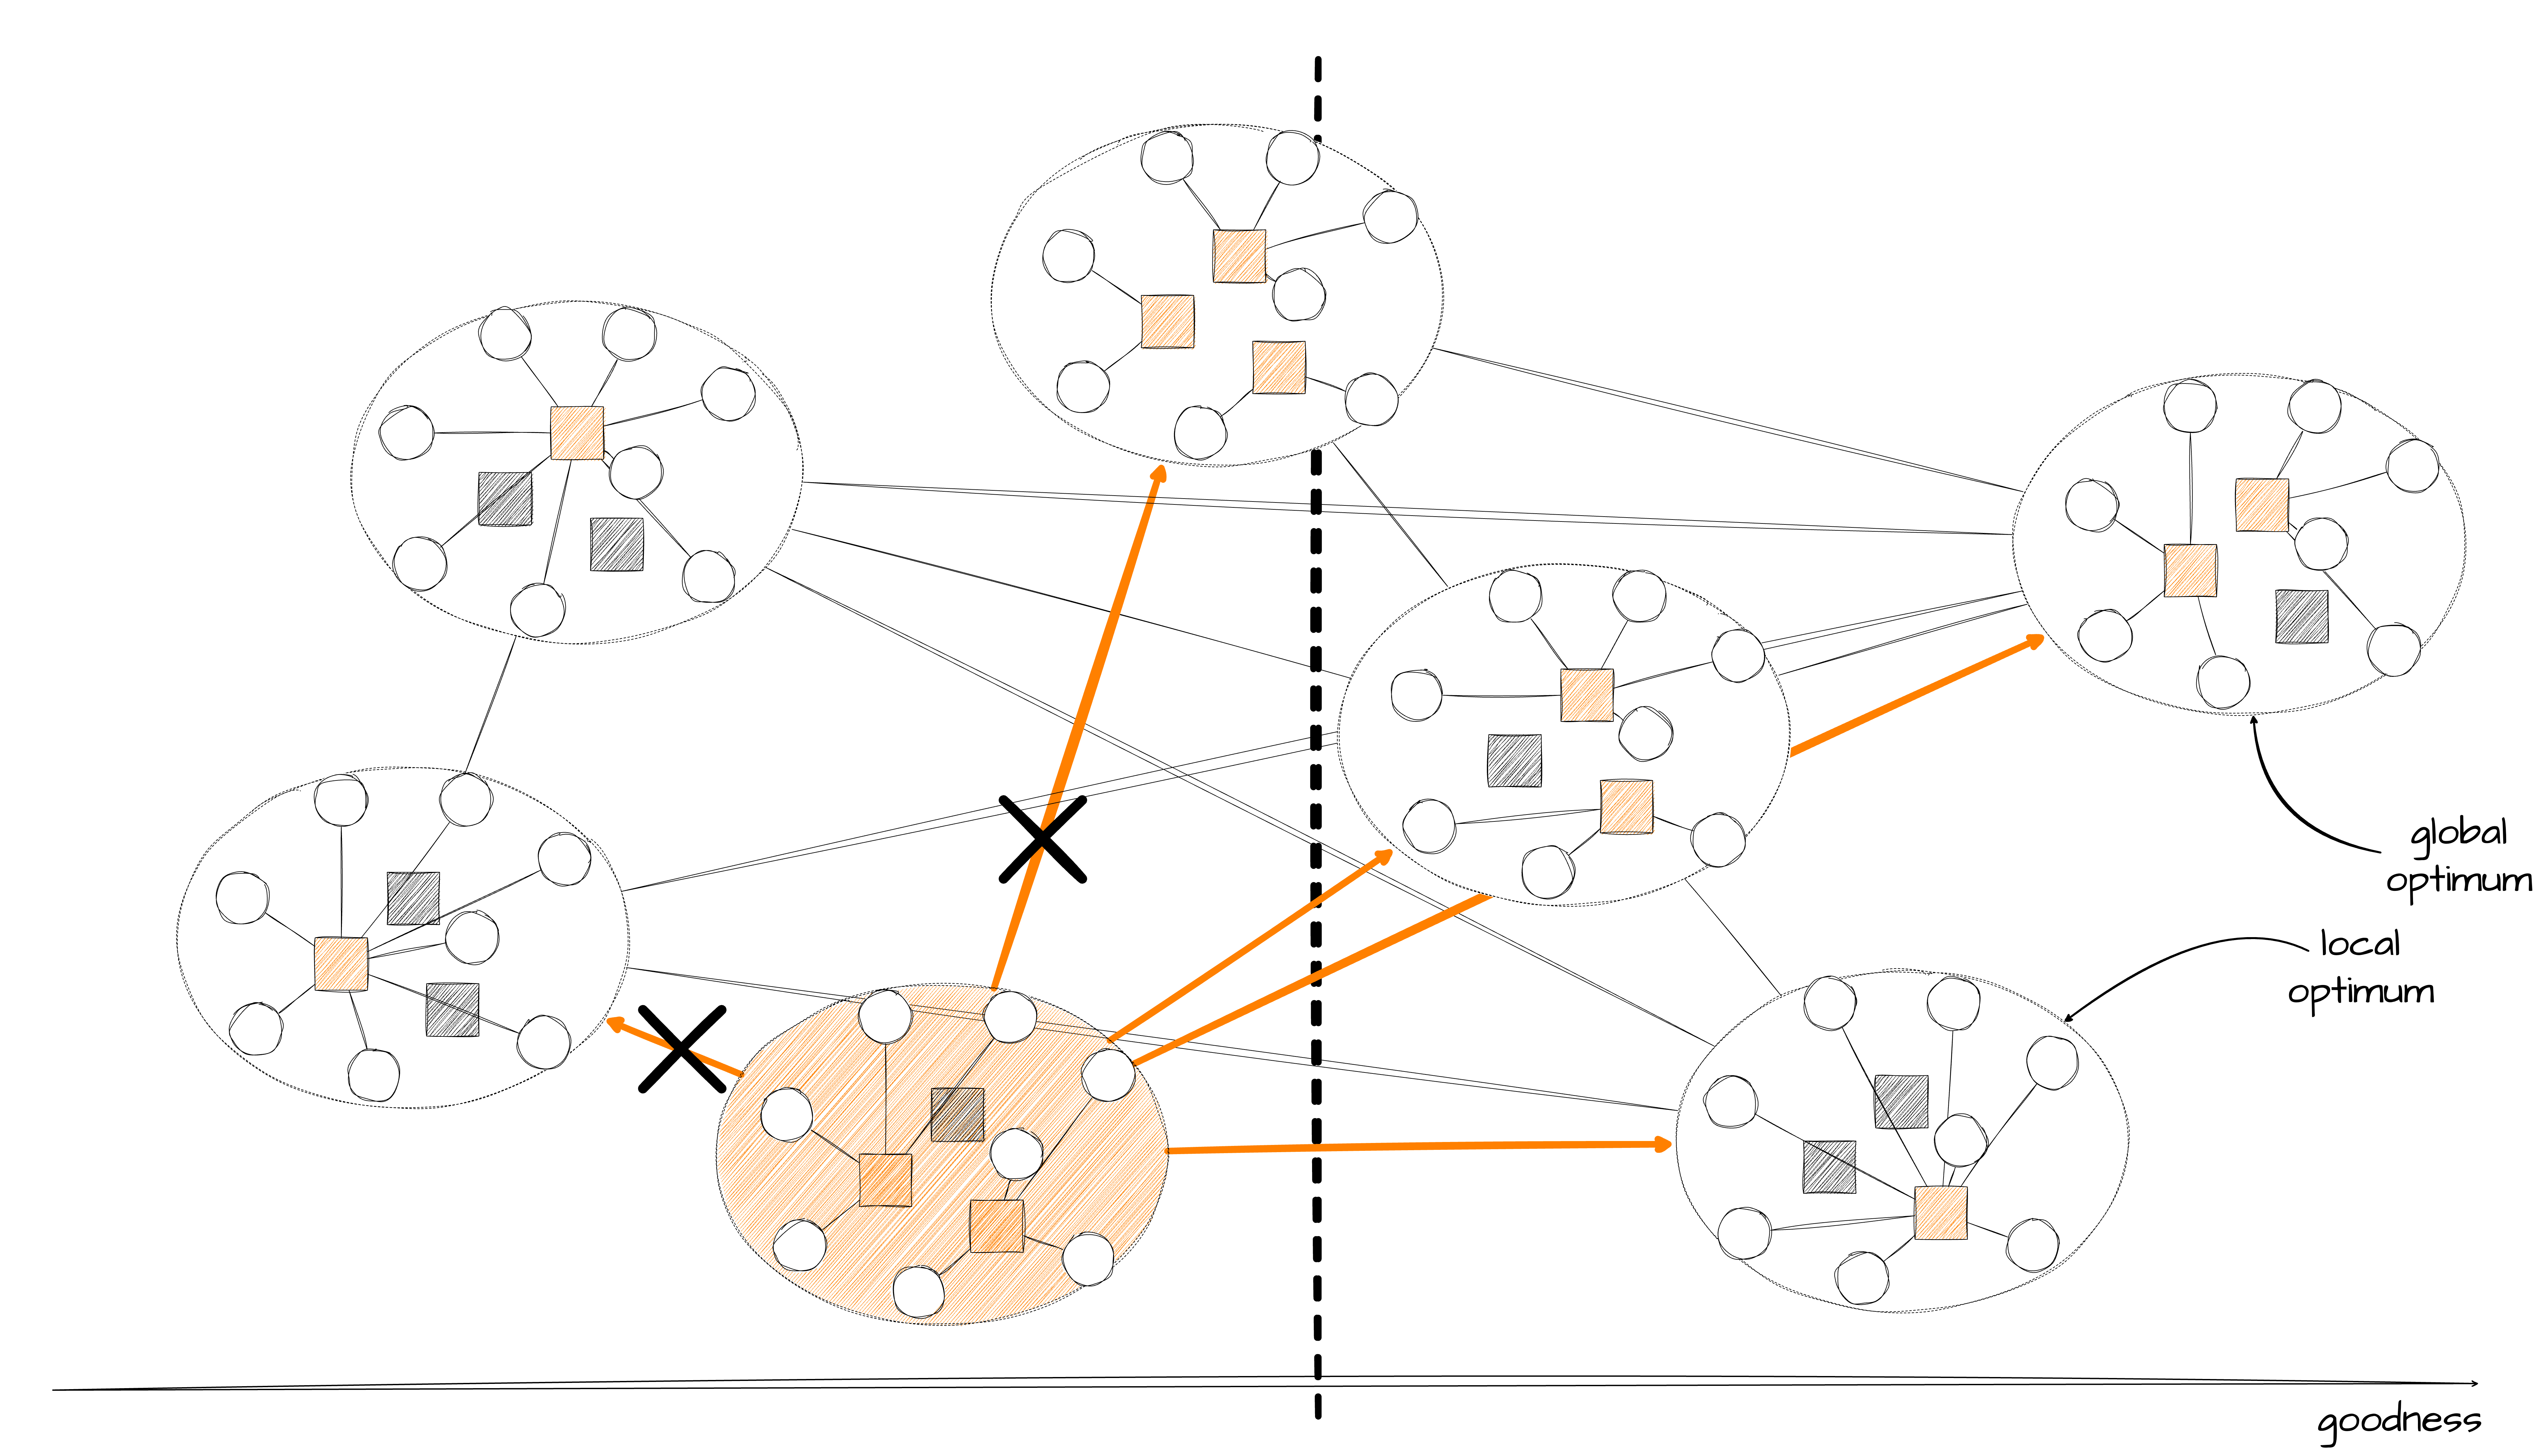
\includegraphics[width=\textwidth]{figures/scheme/thresholded-moving.drawio.png}
      \end{figure}
    \end{column}
  \end{columns}

  \note{
    \begin{itemize}
      \item これから 2 つの改良アイデアを別個に説明する、その後にこれらを問題なく組み合わせられることを説明する
    \end{itemize}
  }
\end{frame}

\begin{frame}{改良点①：開設コストのスケーリング}
  \begin{itemize}
    \item 任意の定数 \(\mu > 0\) に対し、各施設 \(i\) の開設コストを \( \alert{f'_{i} = f_i / \mu} \) でスケール
    \item スケーリング後の開設コスト \(f'_{i}\) を用いて局所探索アルゴリズムを実行
    \item 得られた解をそのまま元のインスタンスの解として出力
  \end{itemize}

  \begin{lemma}[開設コストのスケーリングによる近似比の改善]
    スケーリングによって得られた解の総コストは高々 \((1 + \sqrt{2})\OPT\) である。
  \end{lemma}
\end{frame}

\begin{frame}{改良点①：近似比の解析の概要}

  \only<1>{
    \begin{tikzpicture}[
        box/.style={
            draw,
            rectangle,
            align=center,
            inner sep=6pt
          },
        decoration=penciline,
        >=Latex
      ]

      % -------------------------------------------------
      % horizontal separator (instance boundary)
      % -------------------------------------------------
      \draw[decorate, densely dotted, thick] (-9,1.5) -- (5,1.5);

      \useasboundingbox (-3, -2) rectangle (6, 5);

      \node[anchor=east] at (-3.4,1.9) {\small{元のインスタンス \(\mathcal{I = (\FacilitySet, \DemandSet)}\)}};
      \node[anchor=east] at (-3.4,1.1) {\small{変換後のインスタンス \(\mathcal{I}' = (\FacilitySet', \DemandSet)\)}};

      % -------------------------------------------------
      % boxes (top: I)
      % -------------------------------------------------
      \node[decorate, box] (Isol) at (2.5,4) {
        \(\mathcal{I}\) の実行可能解\\
        割り当てコスト: $C$\\
        配置コスト: $\mu F$
      };

      % -------------------------------------------------
      % boxes (bottom: I')
      % -------------------------------------------------
      \node[decorate, box] (Ilocal) at (2.5,-0.5) {
        \(\mathcal{I}'\) の局所最適解\\
        割り当てコスト: $C$\\
        配置コスト: $F$
      };

      % -------------------------------------------------
      % arrows (reinterpretation)
      % -------------------------------------------------
      \draw[->, decorate] (Ilocal) -- node[right] {再解釈} (Isol);

      \draw[<-, decorate]
      (Isol.west) -- ++(-2.5,0)
      node[left] {出力する};

      \draw[<-, decorate]
      (Ilocal.west) -- ++(-2.5,0)
      node[left] {求める};

    \end{tikzpicture}
  }

  \only<2>{
    \begin{tikzpicture}[
        box/.style={
            draw,
            rectangle,
            align=center,
            inner sep=6pt
          },
        decoration=penciline,
        >=Latex
      ]

      % -------------------------------------------------
      % horizontal separator (instance boundary)
      % -------------------------------------------------
      \draw[decorate, densely dotted, thick] (-9,1.5) -- (5,1.5);

      \useasboundingbox (-3, -2) rectangle (6, 5);

      \node[anchor=east] at (-3.4,1.9) {\small{元のインスタンス \(\mathcal{I = (\FacilitySet, \DemandSet)}\)}};
      \node[anchor=east] at (-3.4,1.1) {\small{変換後のインスタンス \(\mathcal{I}' = (\FacilitySet', \DemandSet)\)}};

      % -------------------------------------------------
      % boxes (top: I)
      % -------------------------------------------------
      \node[decorate, box] (Iopt) at (-2.5,4) {
        \(\mathcal{I}\) の最適解\\
        割り当てコスト: $C^*$\\
        配置コスト: $F^*$
      };

      \node[decorate, box] (Isol) at (2.5,4) {
        \(\mathcal{I}\) の実行可能解\\
        割り当てコスト: $C$\\
        配置コスト: $\mu F$
      };

      % -------------------------------------------------
      % boxes (bottom: I')
      % -------------------------------------------------
      \node[decorate, box] (Ioptp) at (-7.5,-0.5) {
        (\(\mathcal{I}'\)の最適解)
      };

      \node[decorate, box] (Ioptp) at (-2.5,-0.5) {
        \(\mathcal{I}'\)の実行可能解\\
        割り当てコスト: $C^*$\\
        配置コスト: $F^*/\mu$
      };

      \node[decorate, box] (Ilocal) at (2.5,-0.5) {
        \(\mathcal{I}'\) の局所最適解\\
        割り当てコスト: $C \alert{\le C^* + F^* / \mu}$\\
        配置コスト: $F \alert{\le 2C^* + F^* / \mu}$
      };

      % -------------------------------------------------
      % arrows (reinterpretation)
      % -------------------------------------------------
      \draw[->, decorate] (Iopt) -- node[right] {再解釈} (Ioptp);
      \draw[->, decorate] (Ilocal) -- node[right] {再解釈} (Isol);

      % -------------------------------------------------
      % curved arrow (local optimality bound)
      % -------------------------------------------------
      \draw[decorate, ->, dashed, bend right=30]
      (Ioptp) to (Ilocal);

      \node (Ilocalub) at (1.2,-2.2) {
        \alert{補題より}
      };
    \end{tikzpicture}
  }

  \note<2>{
    \begin{itemize}
      \item コストの解析のために \(\mathcal{I}\) の最適解を \(\mathcal{I}'\) の実行可能解として再解釈し、この実行可能解を通じて、\(\mathcal{I}'\) の局所最適解のコストを解析する
      \item なお一般に、\(\mathcal{I}'\) の最適解とこの実行可能解は異なることに注意する
      \item 補題を適用すると、\(\mathcal{I}'\) の局所最適解の割り当てコスト \(C\) と配置コスト \(F\) はそれぞれ
            \[
              C \le C^* + F^*/\mu, \quad F \le 2C^* + F^*/\mu
            \]
            を満たす
    \end{itemize}
  }
\end{frame}

\begin{frame}{改良点①：近似比の解析}
  \begin{lemma}[開設コストのスケーリングによる近似比の改善]
    スケーリングによって得られた解の総コストは高々 \((1 + \sqrt{2})\OPT\) である。
  \end{lemma}

  \vskip -1em

  \begin{align*}
    \underbrace{C + \mu F}_{\text{得られた解の総コスト}} & \le (C^* + F^* / \mu) + \mu (2 C^* + F^* / \mu) \\
                                               & = (1 + 2\mu) C^* + (1 + 1/\mu) F^*
  \end{align*}

  右辺の係数の最大値を最小化（係数が均衡）するように \(\mu\) を選ぶ。\(\mu = 1/\sqrt{2}\) のとき、
  \[
    C + \mu F \le (1 + \sqrt{2})(C^* + F^*) = (1 + \sqrt{2})\OPT
  \]
  が得られる。\hfill\qed
\end{frame}

\begin{frame}{改良点②：近傍への移動に閾値を設ける}
  \begin{itemize}
    \item 任意の定数 \(0 < \delta < 1\) に対し、現在の解のコストが \(1 - \delta\) 倍以下になるような\\近傍への移動のみを許可
    \item そのような解が近傍に存在しない場合、アルゴリズムを終了
  \end{itemize}
\end{frame}

\begin{frame}{改良点②：反復回数の解析}
  \begin{block}{反復回数の上界}
    コストが全て整数であると仮定する。
    初期解のコストを \(M\) とすると、反復回数は高々 \(\mathcal{O}(\log{M}/ \delta)\) 回である。
  \end{block}

  \begin{columns}[T]
    \begin{column}{0.42\textwidth}
      \textbf{Proof. }
      \(k\) を \(M (1-\delta)^k < 1\) を満たす整数とする。

      \only<1>{
        最適解のコストが \(0\) でない限り、任意の実行可能解のコストは少なくとも \(1\) であるため、
        \alert{高々 \(k\) 回の反復でアルゴリズムは停止}する。

        \[
          \text{実際の反復回数} < k
        \]
      }

      \only<2>{
        上式を満たす最小の整数 \(k_{\min}\) について考える。
        \[
          k_{\min} = \left\lceil \frac{\log{M}}{-\log{(1 - \delta)}} \right\rceil \le \frac{\log{M}}{\delta}
        \]
        となるため、\\\alert{反復回数は高々 \(\frac{\log{M}}{\delta}\) 回}である。
      }

    \end{column}
    \begin{column}{0.52\textwidth}
      \only<1>{
        \begin{tikzpicture}[
            decoration=penciline,
          ]
          \begin{axis}[
              clip=false,
              domain=-1:10,
              samples=100,
              axis lines=middle,
              xtick={0, 9},
              xticklabels={0, \(k\)},
              xlabel={\(i\)},
              xlabel style={
                  at={(axis description cs:0.95,0.03)},
                  anchor=north
                },
              ytick={0, 2, 15},
              yticklabels={0, \(1\), \(M\)},
              ylabel={\small{解のコスト}},
              ymin=-1,
              xmax=10.5,
              xmin=-1.2,
              width=8cm,
              height=6cm,
            ]
            \addplot[mark size=0.5pt] {15 * pow(0.75, x)} node[
              pos=0,
              font=\small,
              anchor=south
            ] {$M(1-\delta)^i$};

            \addplot[mark size=0.5pt, dashed, domain=0:10] {2};
            \addplot[only marks, mark=*] coordinates{(0, 15) (0.5, 11) (1, 9) (1.5, 7.5) (2, 5.5) (2.5, 4.5) (3, 3.5)};
            \node[font=\small] at ([yshift=-3mm]current axis.south) {反復回数};

            \draw[<-, decorate]
            (axis cs:3.2,3.6)
            -- ++(20.2,10.5)
            node[right, font=\small] {実際に停止した解};

            \draw[<-, decorate]
            (axis cs:0.5,{15 * pow(0.75, 0.5)})
            -- ++(15,15)
            node[right, font=\small]
              {\(i\) 回反復後の解のコストの上界};
          \end{axis}
        \end{tikzpicture}
      }
      \only<2>{
        \begin{tikzpicture}[
            decoration=penciline,
          ]
          \begin{axis}[
              clip=false,
              domain=-1:10,
              samples=100,
              axis lines=middle,
              xtick={0, 7.5},
              xticklabels={0, \(\quad k\leftarrow\)},
              xlabel={\(i\)},
              xlabel style={
                  at={(axis description cs:0.95,0.03)},
                  anchor=north
                },
              ytick={0, 2, 15},
              yticklabels={0, \(1\), \(M\)},
              ylabel={\small{解のコスト}},
              ymin=-1,
              xmax=10.5,
              xmin=-1.2,
              width=8cm,
              height=6cm,
            ]
            \addplot[mark size=0.5pt] {15 * pow(0.75, x)} node[
              pos=0,
              font=\small,
              anchor=south
            ] {$M(1-\delta)^i$};

            \addplot[mark size=0.5pt, dashed, domain=0:10] {2};
            \addplot[only marks, mark=*] coordinates{(0, 15) (0.5, 11) (1, 9) (1.5, 7.5) (2, 5.5) (2.5, 4.5) (3, 3.5)};
            \node[font=\small] at ([yshift=-3mm]current axis.south) {反復回数};

            \addplot[mark=*, only marks] coordinates{(7, 2)};
            \draw[<-, decorate]
            (axis cs:7,2)
            -- ++(0,30.5)
            node[anchor=south, font=\small] {\(k\) の下界 \(\frac{\log{M}}{-\log{(1 - \delta)}}\)};

            \draw[<-, decorate]
            (axis cs:0.5,{15 * pow(0.75, 0.5)})
            -- ++(15,15)
            node[right, font=\small]
              {\(i\) 回反復後の解のコストの上界};
          \end{axis}
        \end{tikzpicture}
      }
    \end{column}
  \end{columns}

  \note<2>{
    \begin{itemize}
      \item より正確には実際に起こり得る反復回数の上界
    \end{itemize}

  }
\end{frame}

\begin{frame}{改良点②：近似比解析への影響}
  \begin{block}{反復終了時の解の近似比}
    反復終了時の解の総コストは高々 \(3 / (1 - 2\delta|\FacilitySet|) \times \OPT\) である。
  \end{block}

  \textbf{Sketch of the Proof. }
  \only<1>{
    \begin{block}{3 近似の証明のキーアイデア}
      局所最適解を任意の近傍解と比較したとき、
      \[
        \text{(施設の開閉に伴うコストの変化)} + \text{(割り当ての変化に伴うコスト)} \alert{\ge 0}
      \]
    \end{block}
    この不等式を用いて次の不等式を得た。
    \begin{align*}
      F^* - C + C^*  & \ge 0 \\
      F^* - F + 2C^* & \ge 0
    \end{align*}
  }

  \only<2>{
    \begin{block}{改良点② における解析}
      反復終了時の解を任意の近傍解と比較したとき、
      \begin{align*}
         & \text{(施設の開閉に伴うコストの変化)} + \text{(割り当ての変化に伴うコスト)} \\
         & \alert{\ge - \delta \cdot \text{(反復終了時の解のコスト)}}
      \end{align*}
    \end{block}
    この不等式を用いて
    \begin{align*}
      F^* - C + C^*  & \ge -\delta (F + C) \times \text{(最適解の施設数)} \ge - \delta |\FacilitySet| (F + C)         \\
      F^* - F + 2C^* & \ge -\delta (F + C) \times \text{(反復終了時の解と最適解の施設数)} \ge - \delta |\FacilitySet| (F + C)
    \end{align*}
  }

  \only<3>{
    \begin{align*}
      F^* - C + C^*  & \ge - \delta |\FacilitySet| (F + C) \\
      F^* - F + 2C^* & \ge - \delta |\FacilitySet| (F + C)
    \end{align*}

    これらを足し合わせて整理すると、
    \[
      (1 - 2\delta|\FacilitySet|) (F + C) \le 3C^* + 2F^* \le 3 \OPT
    \]
    が得られる。\hfill\qed
  }

\end{frame}

\begin{frame}{改良点②：近傍への移動に閾値を設ける}
  \begin{block}{反復回数の上界}
    コストが全て整数であると仮定する。
    初期解のコストを \(M\) とすると、反復回数は高々 \(\mathcal{O}(\log{M}/ \delta)\) 回である。
  \end{block}

  \begin{block}{反復終了時の解の近似比}
    反復終了時の解の総コストは高々 \(3 / (1 - 2\delta|\FacilitySet|) \times \OPT\) である。
  \end{block}

  \(\epsilon\) を定数として、\(\delta = \epsilon / (2|\FacilitySet|)\) と選ぶ。
  このとき、反復回数は高々 \(\mathcal{O}(|\FacilitySet| \log{M} / \epsilon)\) 回で、反復終了時の解の近似比は高々 \(3 + \epsilon\) 倍である。

  \begin{theorem}[\cite{charikar2005improved}]
    施設配置問題に対して，任意の定数 \(\varepsilon > 0\) に対し，
    % \alert{\(\tilde{\mathcal{O}}(n^2/\varepsilon)\)} 
    入力と \(1/\varepsilon\) の多項式時間で \alert{\(1 + \sqrt{2} + \varepsilon\)} 倍の近似解を求めるスキームが存在する．
  \end{theorem}
\end{frame}

